\section{Part 2 -- Alternative Architecture and Analysis}

\subsection{Alternative Architecture}

As an alternative to the previously proposed model, we developed a model of a system that functions without the Communication Devices.
For this, the Sensor Units received additional communication capabilities (Bluetooth, wi-fi and GPRS) and the Sensor Network was restructured.

The goal of this alternative is to reduce overall latency by reducing the number of hops data needs to take.
The disadvantage of this approach is that the Sensor Units could become more expensive to produce and the ability to send data over a wired connection is lost.

The remainder of the system remains intact. 

\begin{figure}[h]
\caption{Structure of the alternative Sensor Network}
\label{fig:sensornetworkalt}
\centering
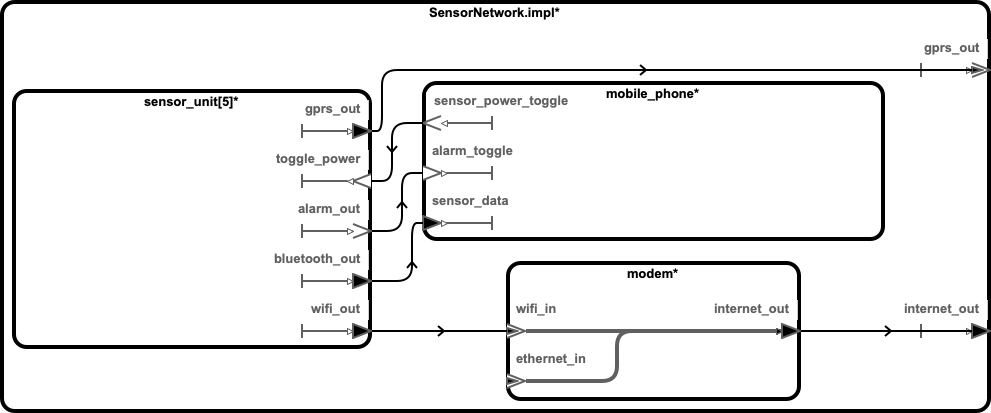
\includegraphics[width=0.45\textwidth]{SensorNetworkAlt}
\end{figure}

\begin{figure}[h]
\caption{Internal structure of an alternative Sensor Unit}
\label{fig:sensorunitalt}
\centering
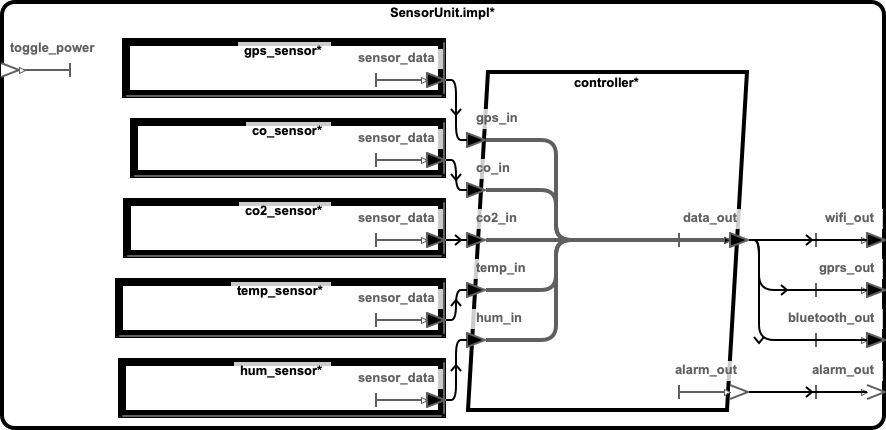
\includegraphics[width=0.45\textwidth]{SensorUnitAlt}
\end{figure}

\subsection{Architectural Analysis}

The AADL model allows us to perform several types of analyses on the system. For the purposes of this assignment, we decided to focus on the flow latency analysis, which seems particularly relevant in the context of a fire alarm system. When it comes to emergencies, response time is crucial, and the system latency can directly impact the agility of emergency services.

In order to perform this analysis, we added flow sources, sinks and paths to our AADL model. Devices that produce data are flow sources, and devices which consume data are flow sinks. Other devices, which only transcode and transmit data, are flow paths. 

Since our system has three primary levels of abstraction, flow sources, sinks and paths had to be added in each one. For example: a Sensor device is a flow source within the context of a Sensor Unit, but the Sensor Unit is the flow source within the context of the Sensor Network, which is itself a flow source within the context of the whole system.

A similar structure applies to flow sinks and paths, which are also present within several layers. Once all sources, sinks and paths are defined, an *end to end flow* is declared, allowing us to perform flow latency analysis on the pairs of sources and sinks are interesting to us.

Since we do not have real world latency values for each communication technology within this context, path latencies were estimated according to general specifications of each technology.

\subsection{Results}

\autoref{fig:rplot02} shows the results of the flow latency analysis, with the minimum and maximum latencies in each flow. The end to end flows analyzed are as follows:

\begin{itemize}
	\item \texttt{etef\_sensor\_phone} and \texttt{etef\_sensor\_phone2}: measure the time it takes for sensor data to reach a Mobile Phone using the first and second Communication Devices, respectively;
	\item \texttt{etef\_sensor\_alarm\_phone} and \texttt{etef\_sensor\_alarm2\_phone}: measure the time it takes for an alert signal produced by the first and second Communication Devices, respectively, to reach a Mobile Phone;
	\item \texttt{etef\_gprs\_db}, \texttt{etef\_ethernet\_db} and \texttt{etef\_wifi\_db}: measure the time it takes for sensor data to reach the Database in the Control Center, for each communication technology; and
	\item \texttt{etef\_gprs\_alarm}, \texttt{etef\_ethernet\_alarm} and \texttt{etef\_wifi\_alarm}: measure the time it takes for an alert signal produced by a Communication Device to reach the Alarm in the Control Center, for each communication technology.
\end{itemize}

\begin{figure}[h]
\caption{Results of the flow latency analysis}
\label{fig:rplot02}
\centering
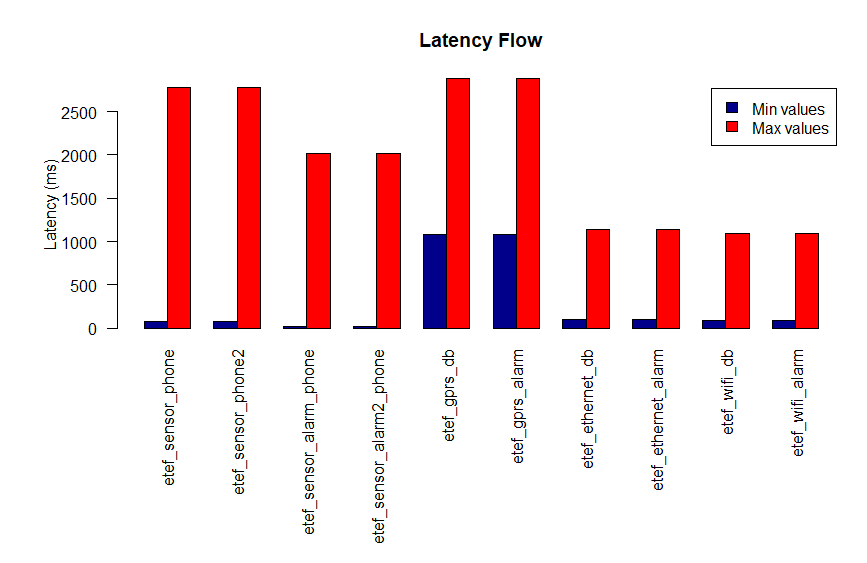
\includegraphics[width=0.45\textwidth]{Rplot02}
\end{figure}

As we can see, there tends to be a large difference between the minimum and maximum latencies, caused by the variable latency in the communication methods and also by the processing time of the data combination thread. Since the thread runs at an interval of 100ms, in the best-case scenario, data reaches the thread immediately before it is executed. On the other hand, if it reaches the thread shortly after execution, the data will only be sent in the next execution 100ms later.

Additionally, we can see that GPRS is the only communication technology with notably greater latency. GPRS signal is sent directly from a Communication Device to a Cell Tower, but it is a slower communication method in general.

Furthermore, an analysis was performed in order to find which ports are used more frequently as flow source or sinks, showing which components are considered crucial to the functioning of the system. \autoref{fig:source} shows the number of times ports are used as flow sources; while \autoref{fig:sink} shows the number of times ports are used as flow sinks.

\begin{figure}[h]
\caption{Ports used as flow sources}
\label{fig:source}
\centering
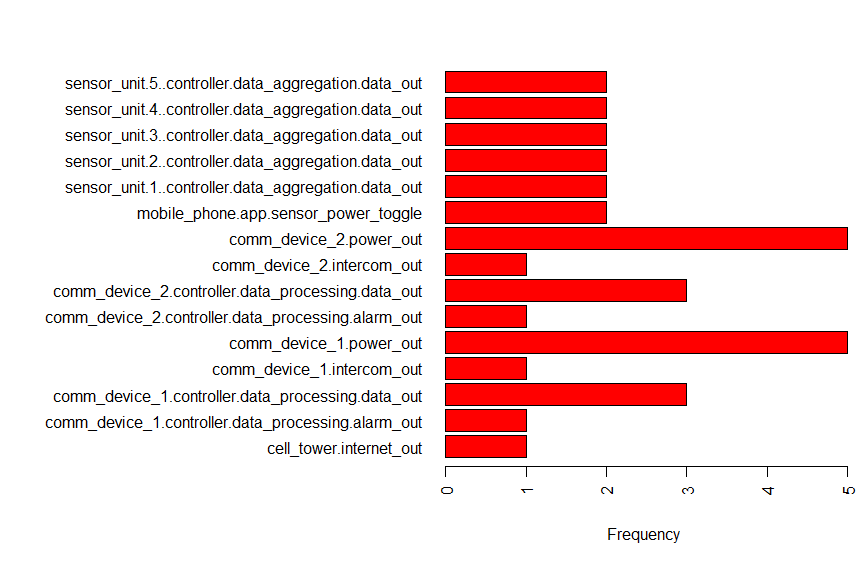
\includegraphics[width=0.45\textwidth]{source}
\end{figure}

\begin{figure}[h]
\caption{Ports used as flow sinks}
\label{fig:sink}
\centering
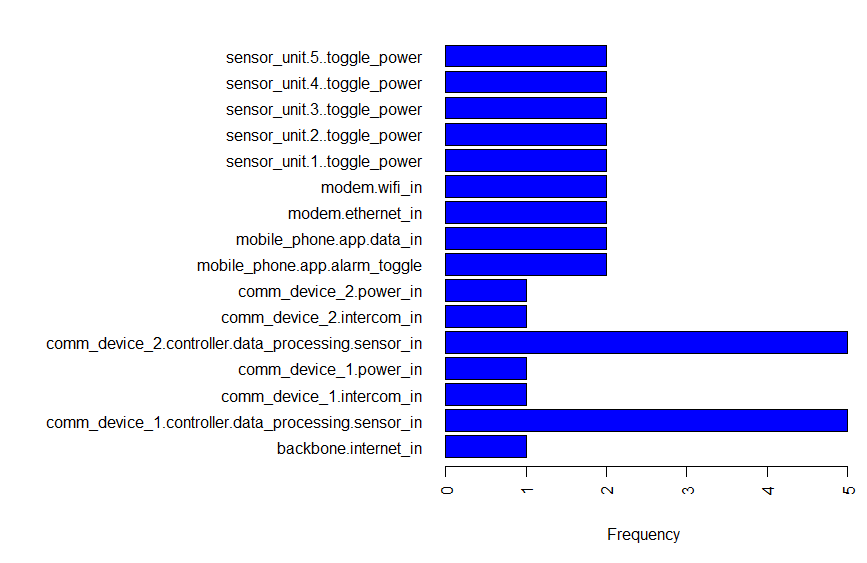
\includegraphics[width=0.45\textwidth]{sink}
\end{figure}


In comparison, \autoref{fig:rplot03} shows the results of the flow latency analysis for the alternative model proposed, with the following flows:

\begin{itemize}
	\item \texttt{etef\_sensor\_phone} and \texttt{etef\_sensor\_alarm\_phone}: measure the time it takes for sensor data or an alert signal to reach a Mobile Phone, respectively;
	\item \texttt{etef\_gprs\_db} and \texttt{etef\_wifi\_db}: measure the time it takes for sensor data to reach the Database in the Control Center, for each communication technology;
	\item \texttt{etef\_gprs\_alarm} and \texttt{etef\_wifi\_alarm}: measure the time it takes for an alert signal produced by a Sensor Unit to reach the Database in the Control Center, for each communication technology;
\end{itemize}

We can see that, by reducing the number of hops in the path, the maximum latencies are much lower. Curiously, with this approach, the GPRS method is faster than Wi-fi, because it avoids the necessity of going through the modem.

\begin{figure}[h]
\caption{Results of the flow latency analysis}
\label{fig:rplot03}
\centering
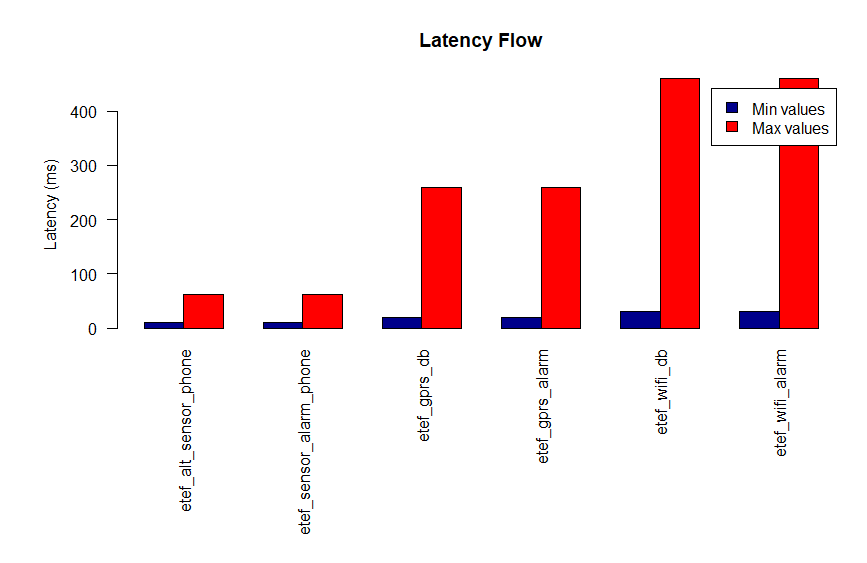
\includegraphics[width=0.45\textwidth]{Rplot03}
\end{figure}

%\limit{6}